\documentclass[11pt,a4paper]{article}

% Packages
\usepackage[utf8]{inputenc}
\usepackage[T1]{fontenc}
\usepackage{amsmath,amssymb,amsthm}
\usepackage{graphicx}
\usepackage{hyperref}
\usepackage{booktabs}
\usepackage{listings}
\usepackage{xcolor}
\usepackage{tikz}
\usetikzlibrary{shapes,arrows,positioning}

% Define Rust language for listings (not built-in)
\lstdefinelanguage{Rust}{
    keywords={fn, let, mut, pub, struct, enum, impl, self, Self, if, else, match, for, while, loop, return, break, continue, where, type, trait, const, static, ref, move, async, await, use, mod, crate, super, in, as, true, false, Ok, Err, Some, None},
    keywordstyle=\color{blue}\bfseries,
    keywords=[2]{u8, u16, u32, u64, u128, i8, i16, i32, i64, i128, f32, f64, bool, char, str, String, Vec, Option, Result, Box, Rc, Arc, H256, AccountId, BlockNumber, BoundedVec, DispatchResult, Error},
    keywordstyle=[2]\color{teal},
    sensitive=true,
    morecomment=[l]{//},
    morecomment=[s]{/*}{*/},
    morestring=[b]",
    morestring=[b]',
}

% Listings configuration
\lstset{
    language=Rust,
    basicstyle=\ttfamily\small,
    keywordstyle=\color{blue}\bfseries,
    commentstyle=\color{gray},
    stringstyle=\color{red!70!black},
    numbers=left,
    numberstyle=\tiny\color{gray},
    breaklines=true,
    frame=single,
    backgroundcolor=\color{gray!5},
    showstringspaces=false,
    tabsize=4
}

% Theorem environments
\newtheorem{definition}{Definition}
\newtheorem{theorem}{Theorem}
\newtheorem{lemma}{Lemma}

% Document info
\title{Augmented Democracy as a Coherence-Constrained Control System\\
\large From Oracle Governance to Quantum-Safe Democratic Infrastructure}

\author{Sylvain Cormier\\
Paraxiom Research\\
\texttt{sylvain@paraxiom.org}}

\date{December 2025}

\begin{document}

\maketitle

\begin{abstract}
We present a systems-theoretic framework for democratic governance that treats
legitimacy as the preservation of coherence in decision-making processes rather
than as a direct consequence of majority outcomes.
The framework introduces \emph{epistemic infrastructure}---including token-curated
test grids, dynamic credential NFTs, and bounded voting weights---that restrict
participation to actors who can demonstrate verifiable engagement with relevant
evidence, without assigning semantic authority to the system itself.

Building on prior work in Hamiltonian machine learning (ERLHS), geometric
consensus (Karmonic Mesh), and quantum-safe validation (Proof of Coherence),
we formalize augmented democracy as a control system in which proposals are
state transitions, participants act as distributed sensors with bounded influence,
and acceptance requires satisfaction of both a democratic majority condition and
a coherence threshold measuring process consistency.

We trace the evolution of this framework from early conceptual work (2017),
through EOS-based smart contract implementations, to its current deployment on
the Quantum Harmony blockchain using post-quantum cryptography and quantum
entropy sources. The central claim is that democratic legitimacy is a measurable
property of process quality---independent of specific outcomes---and that governance
systems designed around epistemic admissibility and coherence constraints exhibit
improved resistance to manipulation, Sybil attacks, plutocratic capture, and
coordinated adversarial behavior.
\end{abstract}

\tableofcontents
\newpage

%------------------------------------------------------------------------------
\section{Problem: Democracy Under Adversarial Load}
\label{sec:problem}
%------------------------------------------------------------------------------

Democratic systems face compounding failure modes in the information age:

\begin{enumerate}
    \item \textbf{Unengaged voting}: Participants lack verifiable engagement with proposal-relevant evidence
    \item \textbf{Manipulation}: Coordinated influence campaigns exploit cognitive biases
    \item \textbf{Speed vs.\ legitimacy}: Rapid decisions sacrifice deliberation quality
    \item \textbf{AI-generated influence}: Large language models enable scalable persuasion
    \item \textbf{Quantum-era threats}: Future adversaries with quantum computers can
    retroactively compromise classical cryptographic commitments
\end{enumerate}

These are not political problems. They are \textit{systems failures}---the democratic control
loop lacks adequate filtering, measurement, and stability guarantees.

Traditional responses (education, regulation, fact-checking) address symptoms rather than
architecture. We require a formal framework that treats democracy as critical infrastructure
subject to engineering constraints.

%------------------------------------------------------------------------------
\section{Philosophical Foundations: Artifacts, Not Truth}
\label{sec:philosophy}
%------------------------------------------------------------------------------

Before presenting the technical framework, we establish a critical philosophical
distinction: \textbf{the governance system does not evaluate truth}. It evaluates
\textit{procedural admissibility} of evidence artifacts and \textit{process consistency}
of decision-making.

\subsection{The Semantic Authority Problem}

Any system that claims to determine ``what is true'' faces an infinite regress:
who verifies the verifiers? Classical epistemic gatekeeping (expert panels,
editorial boards, fact-checkers) ultimately rests on institutional authority
that can be captured, corrupted, or contested.

Our framework sidesteps this problem entirely. The system makes no semantic
judgments. It enforces \textit{procedural constraints} on what evidence may be
referenced and measures \textit{statistical properties} of the decision process.

\subsection{Admissible Artifacts}

\begin{definition}[Admissible Fact Artifact]
In this framework, a \emph{fact} is not treated as a semantic claim or assertion,
but as a verifiable artifact with cryptographic provenance.
An artifact is admissible for use in governance processes if it satisfies:
\begin{enumerate}
    \item \textbf{Immutable referenceability}: the artifact can be uniquely
    identified via a hash, DOI, or equivalent content-addressed reference;
    \item \textbf{Authentic issuance}: the artifact is bound to a recognized
    issuer, authority, or origin via digital signatures or equivalent mechanisms;
    \item \textbf{Contextual relevance}: the artifact belongs to an artifact
    class declared relevant for the proposal type under consideration.
\end{enumerate}
No semantic interpretation, truth evaluation, or correctness judgment is
performed by the governance system itself.
\end{definition}

This definition has important consequences:
\begin{itemize}
    \item A peer-reviewed paper is admissible because it has a DOI, is signed by
    a journal, and belongs to the ``scientific literature'' artifact class---not
    because its conclusions are ``true.''
    \item A government report is admissible because it has a document ID, is
    signed by an agency, and belongs to the ``official statistics'' artifact
    class---not because its numbers are ``correct.''
    \item Participants demonstrate engagement with admissible artifacts, not
    agreement with their conclusions.
\end{itemize}

\subsection{Test Grids as Admissibility Registries}

\begin{definition}[Token-Curated Test Grid]
A Token-Curated Test Grid (TCTG) is a governed registry that specifies which
classes of admissible artifacts may be referenced for a given proposal
domain.
Curation decisions are made by participants who stake tokens and are subject to
economic penalties if admitted artifacts are later shown to be malformed,
inauthentic, or procedurally invalid.

Test grids govern \emph{admissibility criteria} (format, provenance, relevance),
not semantic conclusions or interpretations.
\end{definition}

\textbf{Critical distinction}: Test grids do not define truth; they define the set
of artifacts that a decision process is permitted to reference.

Curators are slashed for admitting artifacts that:
\begin{itemize}
    \item Have invalid provenance (forged signatures, broken hash references)
    \item Violate format requirements (wrong artifact class for proposal type)
    \item Were retracted or invalidated by their issuing authority
\end{itemize}

Curators are \textit{not} slashed for admitting artifacts whose conclusions are
later contested, revised, or overturned through normal scientific or institutional
processes. The system does not adjudicate semantic disputes.

\subsection{Coherence as Process Quality}

\begin{definition}[Process Coherence]
The coherence score $\gamma$ does not measure correctness, factual truth, or
proposal merit. It measures statistical consistency and entropy quality of the
decision process given the declared admissible evidence and participation constraints.

Low coherence indicates process instability, coordinated behavior, or insufficient
entropy, independent of proposal content.
\end{definition}

A proposal can have high coherence and still be ``wrong'' by external standards.
A proposal can have low coherence despite being ``correct.'' The coherence score
measures whether the \textit{process} that produced the decision exhibited
properties consistent with legitimate deliberation.

\subsection{Scope of System Authority}

The governance system constrains \emph{how} decisions are made, not \emph{what}
decisions must conclude.

\begin{center}
\begin{tabular}{ll}
\toprule
\textbf{System Does} & \textbf{System Does Not} \\
\midrule
Verify artifact provenance & Evaluate artifact truth \\
Enforce participation requirements & Determine correct outcomes \\
Measure process consistency & Judge proposal merit \\
Bound individual influence & Override collective judgment \\
Detect coordinated manipulation & Censor unpopular positions \\
\bottomrule
\end{tabular}
\end{center}

This scope limitation is not a weakness but a design requirement. A system that
claimed semantic authority would be both philosophically indefensible and
practically capturable.

%------------------------------------------------------------------------------
\section{Augmented Democracy: Definition}
\label{sec:definition}
%------------------------------------------------------------------------------

\subsection{What Augmented Democracy Is Not}

\begin{itemize}
    \item \textbf{Not technocracy}: Experts do not override participants
    \item \textbf{Not algorithmic rule}: No AI makes final decisions
    \item \textbf{Not censorship}: All proposals enter the system
    \item \textbf{Not plutocracy}: Wealth does not determine influence
    \item \textbf{Not truth arbitration}: The system does not determine what is ``true''
\end{itemize}

\subsection{Definition}

\begin{definition}[Augmented Democracy]
A \textbf{constrained participation system} with admissibility gates, where:
\begin{enumerate}
    \item Participation requires registration (identity binding via dynamic NFTs)
    \item Voters must demonstrate engagement with proposal-relevant admissible artifacts
    \item Proposals traverse a filtering pipeline (review period with gatherers/curators)
    \item Votes are weighted by reputation and bounded by quadratic costs
    \item Acceptance requires coherence threshold satisfaction (process quality)
    \item All transitions produce cryptographic proofs (auditability)
    \item Credentials decay without ongoing participation (life-sustaining NFTs)
\end{enumerate}
\end{definition}

The key distinction from classical democracy: legitimacy derives from \textit{process invariants},
not outcome ratification. The ``augmented'' refers to procedural augmentation---ensuring voters
have verifiably engaged with relevant evidence before their input shapes collective decisions.

%------------------------------------------------------------------------------
% Section: Epistemic Infrastructure (imported)
%------------------------------------------------------------------------------
\section{Procedural Infrastructure: Artifact Curation and Credential Management}
\label{sec:epistemic}

The ``augmented'' in augmented democracy refers not to technological enhancement of voting
mechanics, but to \textit{procedural augmentation}---ensuring that participants have
verifiably engaged with relevant evidence artifacts before their input shapes collective decisions.
This section describes the infrastructure for artifact curation, credential management,
and participation constraints.

\subsection{The Engagement Problem in Democratic Systems}

Classical democratic theory assumes informed voters. Reality provides participants who
may not have engaged with relevant evidence. The augmented democracy framework
addresses this through \textit{mandatory admissibility gates}---structural requirements
that participants demonstrate engagement with proposal-relevant artifacts before voting.

\begin{definition}[Admissibility Gate]
A procedural checkpoint $\mathcal{A}: \mathcal{V} \rightarrow \{0, 1\}$ that maps
a potential voter $v \in \mathcal{V}$ to eligibility status based on demonstrated
engagement with admissible artifacts for the proposal under consideration.
\end{definition}

\textbf{Critical clarification}: This is not a ``literacy test'' or competency filter.
It verifies \textit{engagement with admissible artifacts}, not intelligence, education,
political alignment, or agreement with artifact conclusions. A voter who has engaged
with the relevant evidence and disagrees with its conclusions still passes the gate.

\subsection{Token Curated Test Grids}

The admissibility gate mechanism is implemented through \textbf{Token Curated Test Grids}
(TCTGs), a structure adapted from token curated registries with economic incentives
for quality curation.

As established in Section~\ref{sec:philosophy}, test grids govern \textit{admissibility
criteria}---which artifact classes may be referenced for a proposal domain---not
semantic conclusions or truth claims.

\subsubsection{The Tripartite Structure}

Following the KILT Protocol model~\cite{kilt2020}, TCTGs employ three distinct roles:

\begin{enumerate}
    \item \textbf{Claimer}: A participant who asserts readiness to vote on a proposal
    \item \textbf{Attester}: A curator who has assembled the test grid for that proposal
    \item \textbf{Verifier}: The system (or designated validators) that checks test completion
\end{enumerate}

This separation prevents conflicts of interest: those who create tests do not
administer them, and those who verify do not profit from outcomes.

\subsubsection{Gatherers and Curators}

Within the Attester role, two sub-functions operate:

\begin{itemize}
    \item \textbf{Gatherers}: Identify admissible artifacts for a proposal---documents
    with valid provenance from recognized issuers (scientific journals, government
    agencies, standards bodies). Gatherers are compensated per artifact that meets
    admissibility criteria.

    \item \textbf{Curators}: Assemble gathered artifacts into test grids that verify
    engagement. The goal is to confirm that voters have \textit{encountered} the
    relevant evidence, not that they agree with it. Curators stake tokens on grid quality.
\end{itemize}

\begin{figure}[h]
\centering
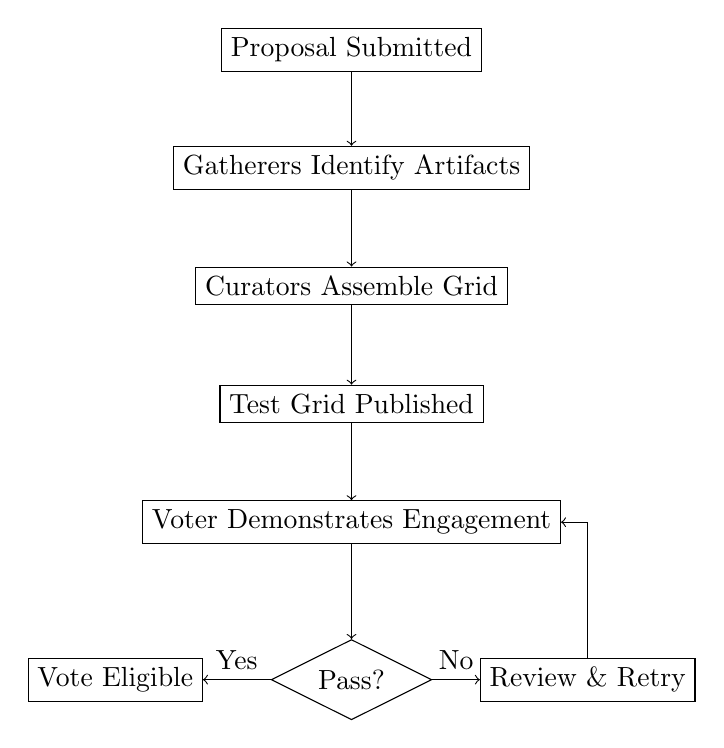
\begin{tikzpicture}[node distance=1.5cm, auto]
    \node[draw, rectangle] (proposal) {Proposal Submitted};
    \node[draw, rectangle, below of=proposal] (gatherers) {Gatherers Identify Artifacts};
    \node[draw, rectangle, below of=gatherers] (curators) {Curators Assemble Grid};
    \node[draw, rectangle, below of=curators] (test) {Test Grid Published};
    \node[draw, rectangle, below of=test] (voter) {Voter Demonstrates Engagement};
    \node[draw, diamond, below of=voter, aspect=2, node distance=2cm] (pass) {Pass?};
    \node[draw, rectangle, left of=pass, node distance=3cm] (eligible) {Vote Eligible};
    \node[draw, rectangle, right of=pass, node distance=3cm] (retry) {Review \& Retry};

    \draw[->] (proposal) -- (gatherers);
    \draw[->] (gatherers) -- (curators);
    \draw[->] (curators) -- (test);
    \draw[->] (test) -- (voter);
    \draw[->] (voter) -- (pass);
    \draw[->] (pass) -- node[above] {Yes} (eligible);
    \draw[->] (pass) -- node[above] {No} (retry);
    \draw[->] (retry) |- (voter);
\end{tikzpicture}
\caption{Token Curated Test Grid Flow}
\label{fig:tctg-flow}
\end{figure}

\subsubsection{Economic Incentives and Slashing Conditions}

Token holders curating test grids face a strategic tension:

\begin{quote}
``Token holders have a tactical incentive to challenge and reject every candidate
to their registry. In the interest of increasing their holdings, this is at odds
with their strategic interest of increasing the value of their holdings. An empty
list is of no interest to consumers.'' --- KILT Protocol
\end{quote}

Applied to TCTGs: curators who create impossible tests drive away voters, reducing
the value of the governance token. Curators who create trivial tests undermine
procedural quality, also reducing token value. The equilibrium favors \textit{fair
tests that accurately verify artifact engagement}.

\textbf{Slashing conditions} (curators lose staked tokens):
\begin{itemize}
    \item Admitting artifacts with invalid provenance (forged signatures, broken hashes)
    \item Admitting artifacts from non-recognized issuers
    \item Admitting artifacts outside the declared artifact class for the proposal domain
    \item Admitting artifacts that were retracted by their issuing authority
\end{itemize}

\textbf{Not slashable} (curators are protected):
\begin{itemize}
    \item Admitting artifacts whose conclusions are later contested or revised
    \item Admitting artifacts that some participants disagree with
    \item Admitting artifacts from one scientific position when others exist
\end{itemize}

The system does not adjudicate semantic disputes. Curators are accountable for
\textit{procedural validity}, not \textit{correctness}.

\subsection{Dynamic NFTs for Credential Management}

Participant credentials in augmented democracy are not static. A voter's eligibility,
weight, and privileges evolve based on contribution history. This is implemented
through \textbf{Dynamic NFTs}---non-fungible tokens whose metadata updates based
on on-chain activity.

\subsubsection{Credential Lifecycle}

\begin{lstlisting}[language=Rust, caption={Dynamic Credential Structure}]
pub struct DynamicCredential<AccountId> {
    pub holder: AccountId,
    pub credential_type: CredentialType,
    pub issued_at: u64,
    pub last_updated: u64,

    // Dynamic fields (updated on-chain)
    pub reputation_score: u64,
    pub proposals_voted: u32,
    pub engagements_verified: u32,  // Test grids passed
    pub engagements_failed: u32,
    pub contributions: u32,
    pub domains_certified: BoundedVec<DomainId, MaxDomains>,

    // Computed eligibility
    pub voting_weight_multiplier: u64,  // basis points
    pub can_submit_proposals: bool,
    pub can_curate_grids: bool,
}

pub enum CredentialType {
    Citizen,        // Basic participation rights
    Contributor,    // Has passed contribution threshold
    Curator,        // Can assemble test grids
    Validator,      // Can verify consensus
    Guardian,       // Emergency governance rights
}
\end{lstlisting}

The credential NFT updates automatically when:
\begin{itemize}
    \item An engagement verification is passed or failed
    \item A vote is cast
    \item A proposal is submitted
    \item Reputation is adjusted by peer review
    \item Domain certification is earned or revoked
\end{itemize}

\subsubsection{Life-Sustaining NFTs}

A critical innovation is the \textbf{Life-Sustaining NFT}---a credential that requires
ongoing activity to remain valid. Unlike static credentials that persist indefinitely,
life-sustaining NFTs decay without continuous participation.

\begin{lstlisting}[language=Rust, caption={Life-Sustaining Credential Logic}]
pub struct LifeSustainingCredential<BlockNumber> {
    pub base_credential: DynamicCredential,
    pub vitality: u64,              // Current life points
    pub max_vitality: u64,          // Maximum life points
    pub decay_rate: u64,            // Points lost per epoch
    pub last_activity: BlockNumber, // Last qualifying action
    pub revival_cost: Balance,      // Cost to revive if expired
}

impl LifeSustainingCredential {
    pub fn is_alive(&self, current_block: BlockNumber) -> bool {
        let epochs_elapsed = (current_block - self.last_activity)
            / EPOCH_LENGTH;
        let decay = epochs_elapsed * self.decay_rate;
        self.vitality > decay
    }

    pub fn sustain(&mut self, activity_points: u64) {
        self.vitality = min(
            self.vitality + activity_points,
            self.max_vitality
        );
        self.last_activity = current_block();
    }
}
\end{lstlisting}

Life-sustaining NFTs address the ``ghost voter'' problem: credentials issued to
participants who subsequently disengage. By requiring periodic activity (voting,
contributing, engagement verification), the system ensures that voting weight reflects
\textit{active} participation, not historical registration.

\subsubsection{Domain-Specific Credentials}

Voters may hold credentials in specific domains:

\begin{center}
\begin{tabular}{ll}
\toprule
\textbf{Domain} & \textbf{Unlocks Voting On} \\
\midrule
Environmental & Climate, conservation, pollution proposals \\
Technical & Infrastructure, protocol upgrades \\
Economic & Treasury, tokenomics, funding proposals \\
Social & Community guidelines, dispute resolution \\
Emergency & Crisis response, security incidents \\
\bottomrule
\end{tabular}
\end{center}

Domain credentials are earned by passing domain-specific engagement verifications and maintained
through ongoing participation in that domain. A participant may hold multiple
domain credentials, each with independent vitality.

\subsection{Quadratic Voting for Bounded Influence}

The augmented democracy framework incorporates \textbf{quadratic voting} to prevent
plutocratic capture while preserving signal strength for high-conviction preferences.

\subsubsection{The Quadratic Cost Function}

The cost to cast $n$ votes on a single proposal from a single participant:

\begin{equation}
    \text{cost}(n) = n^2
\end{equation}

\begin{center}
\begin{tabular}{ccc}
\toprule
\textbf{Votes Cast} & \textbf{Cost} & \textbf{Marginal Cost} \\
\midrule
1 & 1 & 1 \\
2 & 4 & 3 \\
3 & 9 & 5 \\
4 & 16 & 7 \\
5 & 25 & 9 \\
\bottomrule
\end{tabular}
\end{center}

The increasing marginal cost discourages concentration of voting power on single
proposals, encouraging participants to distribute influence across multiple issues.

\subsubsection{Integration with Reputation Weighting}

Quadratic voting combines with reputation-based weighting:

\begin{equation}
    w_{\text{effective}} = \sqrt{\text{votes\_purchased}} \times r_i \times (1 + \epsilon_i)
\end{equation}

where $r_i$ is reputation score and $\epsilon_i$ is the quantum entropy adjustment
from Section~\ref{sec:governance-control}. The square root of purchased votes
ensures diminishing returns, while reputation and entropy preserve the coherence
mechanisms.

\subsubsection{Whale Resistance}

Consider an adversary with 100$\times$ the resources of an average participant:

\begin{center}
\begin{tabular}{lcc}
\toprule
\textbf{System} & \textbf{Adversary Influence} & \textbf{Ratio} \\
\midrule
1-person-1-vote & 1 vote & 1:1 \\
Plutocratic (1:1 stake) & 100 votes & 100:1 \\
Quadratic & 10 votes & 10:1 \\
Quadratic + Reputation Cap & $\leq$ 10 votes & $\leq$ 10:1 \\
\bottomrule
\end{tabular}
\end{center}

Quadratic voting reduces the 100:1 wealth advantage to a 10:1 voting advantage.
Combined with reputation caps and coherence thresholds, adversarial influence
is further bounded.

\subsection{Deliberative Democracy: Multi-Round Consensus}

For high-stakes proposals, the framework supports \textbf{deliberative democracy}
through multiple voting rounds with increasing consensus requirements.

\subsubsection{Unanimity-Seeking Processes}

Drawing from North American Indigenous governance traditions:

\begin{quote}
``Unanimity requires that everyone involved agrees.''
\end{quote}

While perfect unanimity is impractical at scale, the framework supports
\textit{unanimity-seeking} processes:

\begin{enumerate}
    \item \textbf{Round 1}: Simple majority required
    \item \textbf{Round 2}: If Round 1 passes but dissent exceeds threshold,
    deliberation period opens; 60\% supermajority required
    \item \textbf{Round 3}: If significant dissent remains, face-to-face
    (or synchronous digital) deliberation; 75\% required
    \item \textbf{Final Round}: Consensus conference with all registered
    dissenters; 90\% required or proposal modified
\end{enumerate}

This process is expensive and slow---by design. It applies only to proposals
flagged as ``constitutional'' or ``irreversible.''

\subsubsection{Dissent Visibility}

Unlike anonymous voting, deliberative rounds make dissent \textit{visible}
(though not punitive):

\begin{quote}
``Shining the light on someone's disagreement within the consensus could help
the individual and the collective.''
\end{quote}

Visible dissent enables:
\begin{itemize}
    \item Identification of unaddressed concerns
    \item Opportunity for proposal modification
    \item Record of minority positions for future reference
    \item Accountability for officials who override consensus
\end{itemize}

\subsection{Participation History and Accountability}

The system maintains participation history for transparency and accountability,
without claiming to evaluate correctness.

\subsubsection{What Is Recorded}

For each participant:
\begin{itemize}
    \item Engagement verifications passed/failed (procedural record)
    \item Votes cast and their weights (participation record)
    \item Proposals submitted and their outcomes (contribution record)
    \item Coherence scores of votes participated in (process quality record)
\end{itemize}

\subsubsection{What Is Not Recorded or Evaluated}

The system does \textit{not}:
\begin{itemize}
    \item Label votes as ``correct'' or ``incorrect''
    \item Penalize voters for positions that differ from artifact conclusions
    \item Evaluate whether voters ``should have'' voted differently
    \item Assign semantic meaning to voting patterns
\end{itemize}

Participants are free to engage with evidence and reach their own conclusions.
The system verifies engagement, not agreement.

\subsubsection{Official Accountability}

For elected officials, participation history is public record:

\begin{itemize}
    \item Which engagement verifications they passed before voting
    \item How they voted on each proposal
    \item Whether they used override authority
    \item The coherence scores of decisions they participated in
\end{itemize}

This enables informed electoral choices without the system claiming to evaluate
whether official decisions were ``correct.''

\subsection{Node Reputation and Performance History}

The procedural infrastructure includes reputation tracking for \textit{infrastructure
nodes}, not just human participants.

\subsubsection{Oracle Node Reputation}

Nodes providing artifact references (document hashes, provenance data) accumulate
reputation based on:

\begin{itemize}
    \item Availability: Uptime and response latency
    \item Consistency: Variance in reported references
    \item Validity: Proportion of references that pass provenance checks
    \item Longevity: Duration of reliable service
\end{itemize}

This reputation feeds into test grid assembly: artifacts sourced through high-reputation
nodes have verified provenance chains.

\subsubsection{Validator Performance}

Consensus validators are tracked on:

\begin{itemize}
    \item Block production rate
    \item Missed slots
    \item Equivocation incidents
    \item Coherence score contributions
\end{itemize}

Poor-performing validators see reduced block rewards and eventual removal
from the active set.

\subsection{Evolution: EOS to Substrate to Quantum Harmony}

The procedural infrastructure evolved through three phases:

\subsubsection{Phase 1: EOS Smart Contract Prototype (2020--2021)}

Initial implementation as an EOS smart contract:
\begin{itemize}
    \item Basic test grid structure
    \item Token-curated artifact registration
    \item Simple pass/fail admissibility gates
    \item Proof-of-concept dynamic credentials
\end{itemize}

\subsubsection{Phase 2: Substrate Migration (2022--2023)}

Migration to Substrate framework:
\begin{itemize}
    \item Full pallet implementation
    \item NFT-based credential system
    \item Quadratic voting integration
    \item Multi-round deliberation support
\end{itemize}

\subsubsection{Phase 3: Quantum Harmony Integration (2024--2025)}

Current implementation with quantum enhancements:
\begin{itemize}
    \item Quantum entropy for vote weighting (Section~\ref{sec:governance-control})
    \item Post-quantum signatures for credential integrity
    \item Coherence-based consensus replacing stake-based finality
    \item QKD-protected artifact distribution
\end{itemize}

The core procedural architecture---test grids, dynamic credentials, quadratic
voting---persists across all phases. The quantum enhancements provide
cryptographic hardening without altering the democratic logic.

\subsection{Summary: The Procedural Stack}

The complete procedural infrastructure:

\begin{enumerate}
    \item \textbf{Artifact Layer}: Gatherers identify admissible artifacts, nodes verify provenance
    \item \textbf{Test Layer}: Curators assemble grids, token economics enforce quality
    \item \textbf{Credential Layer}: Dynamic NFTs track eligibility, life-sustaining
    requirements enforce engagement
    \item \textbf{Voting Layer}: Quadratic costs bound influence, reputation weights
    signal, entropy randomizes
    \item \textbf{Consensus Layer}: Coherence thresholds measure process quality,
    multi-round processes seek unanimity
    \item \textbf{Accountability Layer}: Participation recorded, officials tracked,
    history immutable
\end{enumerate}

This stack transforms voting from opinion aggregation into \textit{structured
preference revelation}---the foundation of augmented democracy.

\textbf{The system constrains how decisions are made, not what decisions must conclude.}


%------------------------------------------------------------------------------
% Section: Governance as a Control System (imported)
%------------------------------------------------------------------------------
\section{Governance as a Control System}
\label{sec:governance-control}

This section presents a rigorous mapping from classical control theory to democratic governance,
grounded in a production implementation deployed on the Quantum Harmony blockchain. We demonstrate
that democratic processes can be formally modeled as coherence-constrained state machines, where
proposals represent state transitions, participants act as distributed sensors, and legitimacy
emerges from invariant preservation rather than mere majority arithmetic.

\subsection{The Control-Theoretic Frame}

We model a democratic system as a discrete-time control system $\mathcal{G} = (\mathcal{S}, \mathcal{U}, \mathcal{Y}, f, g, \mathcal{C})$ where:

\begin{itemize}
    \item $\mathcal{S}$ is the state space (governance configuration)
    \item $\mathcal{U}$ is the input space (proposals)
    \item $\mathcal{Y}$ is the output space (decisions)
    \item $f: \mathcal{S} \times \mathcal{U} \rightarrow \mathcal{S}$ is the state transition function
    \item $g: \mathcal{S} \rightarrow \mathcal{Y}$ is the output function
    \item $\mathcal{C} \subset \mathcal{S}$ is the coherence manifold---the set of legitimate states
\end{itemize}

The central requirement is \textit{coherence preservation}: for any valid transition $s_{t+1} = f(s_t, u_t)$,
if $s_t \in \mathcal{C}$, then $s_{t+1} \in \mathcal{C}$. Transitions that would exit the coherence
manifold are rejected.

\subsection{Proposals as State Transitions}

In the implementation, proposals are formalized as typed state transition requests with explicit
lifecycle semantics:

\begin{lstlisting}[language=Rust, caption={Proposal Status State Machine (lib.rs:114-124)}]
pub enum ProposalStatus {
    Submitted,        // s_0: Initial state
    UnderReview,      // s_1: Filtering phase
    ReadyForVoting,   // s_2: Cleared for deliberation
    VotingActive,     // s_3: Consensus formation
    VotingClosed,     // s_4: Measurement complete
    Approved,         // s_5+: On-manifold transition accepted
    Rejected,         // s_5-: Off-manifold transition blocked
    QuantumVerified,  // s_6: Cryptographic proof generated
}
\end{lstlisting}

This eight-state machine enforces a strict ordering: $s_0 \rightarrow s_1 \rightarrow s_2 \rightarrow
s_3 \rightarrow s_4 \rightarrow \{s_5^+, s_5^-\} \rightarrow s_6$. The system prohibits state
regression and enforces temporal guards:

\begin{lstlisting}[language=Rust, caption={Temporal Constraints on Voting Phase (lib.rs:430-435)}]
let current_block = <frame_system::Pallet<T>>::block_number();
ensure!(
    current_block >= proposal.voting_starts &&
    current_block <= proposal.voting_ends,
    Error::<T>::ProposalNotInVotingPhase
);
\end{lstlisting}

The \texttt{ReviewPeriod} and \texttt{VotingPeriod} configuration parameters define minimum dwell
times in each phase, preventing rushed transitions that could destabilize the system.

\subsection{Participants as Distributed Sensors}

Democratic participants are modeled as heterogeneous sensors with role-specific measurement capabilities:

\begin{lstlisting}[language=Rust, caption={Participant Roles as Sensor Types (lib.rs:88-94)}]
pub enum ParticipantRole {
    Submitter,   // Proposal origination sensor
    Voter,       // Binary/ternary measurement sensor
    Reviewer,    // Quality filtering sensor
    Validator,   // Consensus verification sensor
}
\end{lstlisting}

Each participant maintains state that influences their measurement weight:

\begin{lstlisting}[language=Rust, caption={Participant State Vector (lib.rs:77-86)}]
pub struct Participant<AccountId> {
    pub account: AccountId,
    pub role: ParticipantRole,
    pub registered_at: u64,
    pub contributions: u64,
    pub reputation: u64,           // Base control gain
    pub quantum_identity: Option<H256>,
}
\end{lstlisting}

The \texttt{reputation} field serves as the base \textit{control gain}---the amplification factor
that determines how strongly a participant's measurement influences the system output. Initial
reputation is set to 100 (lib.rs:336), establishing a baseline that can evolve through contribution history.

\subsection{Deliberation as Filtering}

The review period implements a low-pass filter on the proposal stream:

\begin{lstlisting}[language=Rust, caption={Review Period as Temporal Filter (lib.rs:392-393)}]
voting_starts: <frame_system::Pallet<T>>::block_number()
    + T::ReviewPeriod::get(),
voting_ends: <frame_system::Pallet<T>>::block_number()
    + T::ReviewPeriod::get() + T::VotingPeriod::get(),
\end{lstlisting}

This enforced delay serves multiple control-theoretic purposes:

\begin{enumerate}
    \item \textbf{Noise rejection}: Transient proposals (spam, emotional reactions) decay during the review period
    \item \textbf{Signal integration}: Reviewers accumulate information about proposal quality
    \item \textbf{Aliasing prevention}: The minimum period ensures adequate sampling of community response
\end{enumerate}

The system implements bounded queuing to prevent denial-of-service:

\begin{lstlisting}[language=Rust, caption={Bounded Proposal Queue (lib.rs:366-370)}]
let active_proposals = <Proposals<T>>::iter().count() as u32;
ensure!(
    active_proposals < T::MaxProposals::get(),
    Error::<T>::MaxProposalsReached
);
\end{lstlisting}

\subsection{Credentials as Control Gains}

Vote weight is computed as a function of reputation modulated by quantum entropy:

\begin{lstlisting}[language=Rust, caption={Control Gain Computation (lib.rs:617-631)}]
fn calculate_quantum_vote_weight(
    participant: &Participant<T::AccountId>,
    entropy: &[u8],
) -> Result<u64, Error<T>> {
    // Base weight from reputation
    let base_weight = participant.reputation;

    // Add quantum randomness factor (+/- 10%)
    let entropy_factor = (entropy[0] as u64 % 21) as i64 - 10;
    let quantum_adjustment =
        (base_weight as i64 * entropy_factor) / 100;

    let final_weight =
        (base_weight as i64 + quantum_adjustment).max(1) as u64;

    Ok(final_weight)
}
\end{lstlisting}

This formulation has precise control-theoretic semantics:

\begin{equation}
    w_i = \max\left(r_i + \frac{r_i \cdot (\eta_i \mod 21 - 10)}{100}, 1\right)
\end{equation}

where $w_i$ is the final weight, $r_i$ is the base reputation, and $\eta_i$ is the quantum entropy
byte. The entropy introduces a $\pm 10\%$ perturbation, which serves two purposes:

\begin{enumerate}
    \item \textbf{Sybil resistance}: An attacker controlling multiple identities cannot precisely
    predict aggregate weight
    \item \textbf{Tie-breaking}: Near-equal coalitions are resolved by entropy rather than timestamp
    or insertion order
\end{enumerate}

The \texttt{max(..., 1)} floor ensures no participant has zero influence---a stability constraint
preventing degenerate control configurations.

\subsection{Coherence as System Invariant}

The central contribution is the dual-condition consensus requirement:

\begin{lstlisting}[language=Rust, caption={Coherence-Constrained Consensus (lib.rs:666-667)}]
// Proposal approved if majority approves AND
// quantum confidence is high
let approved = approve_weight > reject_weight
    && quantum_confidence > 50;
\end{lstlisting}

This is not mere majority rule. Approval requires \textit{both}:

\begin{enumerate}
    \item $w_{\text{approve}} > w_{\text{reject}}$ (democratic condition)
    \item $\gamma > 50$ (coherence condition)
\end{enumerate}

where $\gamma$ is the \textit{quantum confidence score}, computed as:

\begin{lstlisting}[language=Rust, caption={Quantum Confidence Computation (lib.rs:679-715)}]
fn calculate_quantum_confidence(
    votes: &[QuantumVote<T::AccountId>],
) -> Result<u32, Error<T>> {
    // ... compute mean entropy across votes ...

    for vote in votes {
        let entropy_value = vote.quantum_nonce.iter()
            .map(|&b| b as f64)
            .sum::<f64>() / vote.quantum_nonce.len() as f64;

        entropy_variance +=
            (entropy_value - mean_entropy).powi(2);
    }

    entropy_variance /= votes.len() as f64;

    // Higher variance indicates better quantum randomness
    let confidence =
        ((entropy_variance / 255.0).min(1.0) * 100.0) as u32;

    Ok(confidence)
}
\end{lstlisting}

The coherence score measures the \textit{quality of the randomness distribution} across votes:

\begin{equation}
    \gamma = \min\left(\frac{\sigma^2_\eta}{255}, 1\right) \times 100
\end{equation}

where $\sigma^2_\eta$ is the variance of mean entropy values across all votes. This captures a
subtle but critical property: a legitimate vote should exhibit high entropy variance (true quantum
randomness), while a coordinated attack (replay, Sybil) will show artificially low variance.

\textbf{Critical clarification}: The coherence score $\gamma$ measures \textit{process quality},
not outcome correctness. A proposal can have high coherence and still be ``wrong'' by external
standards. A proposal can have low coherence despite being ``correct.'' The score measures whether
the \textit{process} exhibited properties consistent with legitimate deliberation---statistical
independence of participants and adequate entropy quality---independent of proposal content.

\textbf{Key insight}: The coherence threshold acts as a Lyapunov function. States with $\gamma \leq 50$
are \textit{outside the coherence manifold}---they may satisfy the democratic condition but fail the
process quality invariant. The system refuses to transition to such states, even under majority pressure.

\subsection{Rejection of Off-Manifold Transitions}

The error handling system explicitly enumerates forbidden transitions:

\begin{lstlisting}[language=Rust, caption={Off-Manifold Action Rejection (lib.rs:273-310)}]
pub enum Error<T> {
    ParticipantNotRegistered,    // Unidentified sensor
    ParticipantAlreadyRegistered,
    ProposalNotFound,            // Invalid reference
    ProposalNotInVotingPhase,    // Temporal violation
    AlreadyVoted,                // Replay attempt
    InsufficientQuantumEntropy,  // Entropy pool exhausted
    InvalidQuantumSignature,     // Authentication failure
    Unauthorized,                // Role violation
    MaxProposalsReached,         // Queue overflow
    MaxVotersReached,            // Capacity limit
    InvalidProposalData,         // Malformed input
    QuantumConsensusFailed,      // Coherence violation
}
\end{lstlisting}

Each error type corresponds to a specific invariant violation:

\begin{center}
\begin{tabular}{ll}
\toprule
\textbf{Error} & \textbf{Violated Invariant} \\
\midrule
\texttt{InsufficientQuantumEntropy} & Resource availability \\
\texttt{ProposalNotInVotingPhase} & Temporal ordering \\
\texttt{AlreadyVoted} & Idempotency \\
\texttt{Unauthorized} & Role-based access \\
\texttt{QuantumConsensusFailed} & Coherence threshold \\
\bottomrule
\end{tabular}
\end{center}

\subsection{Bounded Influence and Stability}

The system enforces hard bounds on participation:

\begin{lstlisting}[language=Rust, caption={Configuration Bounds (lib.rs:46-56)}]
#[pallet::constant]
type MaxProposals: Get<u32>;

#[pallet::constant]
type MaxVoters: Get<u32>;

#[pallet::constant]
type MaxReviewers: Get<u32>;
\end{lstlisting}

These bounds serve as \textit{stability constraints}:

\begin{itemize}
    \item \textbf{MaxProposals}: Prevents unbounded growth of the pending state space
    \item \textbf{MaxVoters}: Limits consensus computation complexity to $O(n)$
    \item \textbf{MinQuantumEntropy}: Ensures sufficient randomness reservoir
\end{itemize}

The entropy pool management (lib.rs:557-574) implements a FIFO queue with bounded capacity:

\begin{lstlisting}[language=Rust, caption={Entropy Pool Constraint (lib.rs:562-565)}]
ensure!(
    pool_size >= bytes &&
    pool_size >= T::MinQuantumEntropy::get(),
    Error::<T>::InsufficientQuantumEntropy
);
\end{lstlisting}

Operations fail gracefully when entropy is exhausted, preventing the system from entering a
low-coherence regime where randomness quality degrades.

\subsection{Cryptographic Proof Generation}

Each consensus produces a verifiable proof:

\begin{lstlisting}[language=Rust, caption={Consensus Proof Generation (lib.rs:718-741)}]
fn generate_quantum_consensus_proof(
    votes: &[QuantumVote<T::AccountId>],
    result: &QuantumConsensusResult,
) -> Result<BoundedVec<u8, ConstU32<1024>>, Error<T>> {
    let mut proof_data = Vec::new();

    // Aggregate vote signatures
    for vote in votes {
        proof_data.extend_from_slice(&vote.quantum_signature);
    }

    // Bind to result
    proof_data.extend_from_slice(&result.encode());

    // Add fresh entropy
    let quantum_entropy = Self::consume_quantum_entropy(64)?;
    proof_data.extend_from_slice(&quantum_entropy);

    // Commit
    let proof = BlakeTwo256::hash(&proof_data);

    Ok(proof.as_bytes().to_vec().try_into()?)
}
\end{lstlisting}

This proof commits to:
\begin{enumerate}
    \item All individual vote signatures (participation record)
    \item The computed result (outcome binding)
    \item Fresh quantum entropy (temporal uniqueness)
\end{enumerate}

The resulting Blake2-256 hash provides a succinct, collision-resistant commitment that can be
verified without reconstructing the full vote set.

\subsection{Summary: The Control Loop}

The complete governance control loop is:

\begin{enumerate}
    \item \textbf{Input}: Proposal $u_t$ submitted by registered Submitter
    \item \textbf{Filtering}: Review period applies temporal low-pass filter
    \item \textbf{Measurement}: Voters provide weighted observations $\{(v_i, w_i)\}$
    \item \textbf{Aggregation}: Compute $w_{\text{approve}}, w_{\text{reject}}, w_{\text{abstain}}$
    \item \textbf{Coherence Check}: Compute $\gamma$ from entropy distribution
    \item \textbf{Decision}: Accept transition iff $w_{\text{approve}} > w_{\text{reject}} \land \gamma > 50$
    \item \textbf{Proof}: Generate cryptographic commitment to decision
    \item \textbf{State Update}: Transition to $s_{t+1}$ or reject and remain at $s_t$
\end{enumerate}

\begin{figure}[h]
\centering
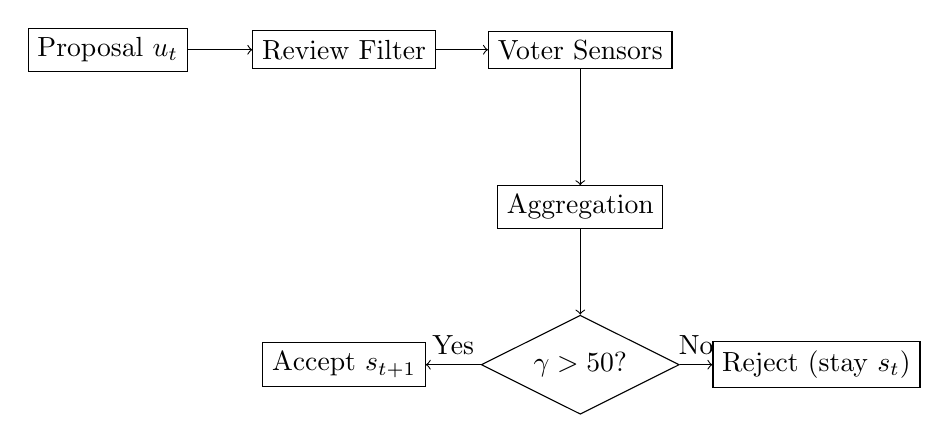
\begin{tikzpicture}[node distance=2cm, auto]
    \node[draw, rectangle] (input) {Proposal $u_t$};
    \node[draw, rectangle, right of=input, node distance=3cm] (filter) {Review Filter};
    \node[draw, rectangle, right of=filter, node distance=3cm] (sensors) {Voter Sensors};
    \node[draw, rectangle, below of=sensors] (aggregate) {Aggregation};
    \node[draw, diamond, below of=aggregate, aspect=2] (coherence) {$\gamma > 50$?};
    \node[draw, rectangle, left of=coherence, node distance=3cm] (accept) {Accept $s_{t+1}$};
    \node[draw, rectangle, right of=coherence, node distance=3cm] (reject) {Reject (stay $s_t$)};

    \draw[->] (input) -- (filter);
    \draw[->] (filter) -- (sensors);
    \draw[->] (sensors) -- (aggregate);
    \draw[->] (aggregate) -- (coherence);
    \draw[->] (coherence) -- node[above] {Yes} (accept);
    \draw[->] (coherence) -- node[above] {No} (reject);
\end{tikzpicture}
\caption{Governance Control Loop with Coherence Gate}
\label{fig:control-loop}
\end{figure}

The critical observation is that the coherence gate ($\gamma > 50$) is \textit{not optional}.
Even unanimous approval fails if the entropy distribution indicates manipulation. This inverts
the traditional democratic assumption: legitimacy is not derived from majority agreement, but
from the quality of the process that produced the agreement.

\subsection{Implications for Democratic Theory}

This control-theoretic framing has several implications:

\begin{enumerate}
    \item \textbf{Legitimacy is measurable}: The coherence score $\gamma$ provides a quantitative
    measure of process quality, independent of outcome.

    \item \textbf{Manipulation is detectable}: Coordinated attacks produce low-variance entropy
    distributions, triggering coherence failure before state corruption.

    \item \textbf{Stability is guaranteed}: Bounded queues, temporal guards, and entropy floors
    prevent the system from entering degenerate configurations.

    \item \textbf{Rollback is possible}: Rejected transitions leave the system at $s_t$, enabling
    retry with improved proposals rather than corrupted state recovery.
\end{enumerate}

The implementation demonstrates that coherence-constrained democratic systems are not merely
theoretical constructs but deployable infrastructure with formal guarantees.

\subsection{Scope of Control}

A final clarification on system scope:

\textbf{The governance system constrains how decisions are made, not what decisions must conclude.}

The control system ensures:
\begin{itemize}
    \item Participants have engaged with admissible artifacts (procedural gate)
    \item Influence is bounded and distributed (quadratic costs, reputation caps)
    \item The decision process exhibits statistical independence (coherence threshold)
    \item All transitions are auditable (cryptographic proofs)
\end{itemize}

The control system does \textit{not} ensure:
\begin{itemize}
    \item Outcomes are ``correct'' by any external standard
    \item Participants agree with artifact conclusions
    \item Proposals are wise, beneficial, or optimal
    \item The collective makes ``good'' decisions
\end{itemize}

This scope limitation is deliberate. A system that claimed to guarantee correct outcomes would
require semantic authority---the ability to evaluate truth---which is both philosophically
indefensible and practically capturable. By limiting scope to process quality, the system
remains defensible as infrastructure rather than oracle.


%------------------------------------------------------------------------------
% Section: The Coherence Pipeline (bridge section)
%------------------------------------------------------------------------------
\section{The Coherence Pipeline: From Question to Result}
\label{sec:pipeline}

The preceding sections describe components. This section shows how they integrate
into a single coherent pipeline. The augmented democracy system is not a collection
of mechanisms but a \textit{processing pipeline} where each stage gates the next.

\subsection{The Six-Stage Pipeline}

\begin{figure}[ht]
\centering
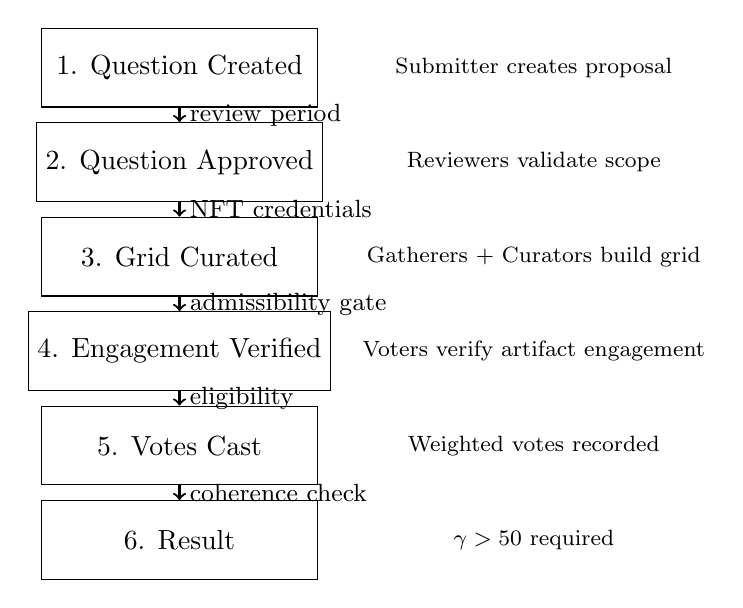
\begin{tikzpicture}[
    node distance=1.2cm,
    stage/.style={draw, rectangle, minimum width=3.5cm, minimum height=1cm, align=center},
    arrow/.style={->, thick}
]
    % Stages
    \node[stage] (q) {1. Question Created};
    \node[stage, below of=q] (a) {2. Question Approved};
    \node[stage, below of=a] (g) {3. Grid Curated};
    \node[stage, below of=g] (t) {4. Engagement Verified};
    \node[stage, below of=t] (v) {5. Votes Cast};
    \node[stage, below of=v] (r) {6. Result};

    % Arrows with labels
    \draw[arrow] (q) -- node[right, font=\small] {review period} (a);
    \draw[arrow] (a) -- node[right, font=\small] {NFT credentials} (g);
    \draw[arrow] (g) -- node[right, font=\small] {admissibility gate} (t);
    \draw[arrow] (t) -- node[right, font=\small] {eligibility} (v);
    \draw[arrow] (v) -- node[right, font=\small] {coherence check} (r);

    % Side annotations
    \node[right of=q, node distance=4.5cm, font=\footnotesize, align=left] {Submitter creates proposal};
    \node[right of=a, node distance=4.5cm, font=\footnotesize, align=left] {Reviewers validate scope};
    \node[right of=g, node distance=4.5cm, font=\footnotesize, align=left] {Gatherers + Curators build grid};
    \node[right of=t, node distance=4.5cm, font=\footnotesize, align=left] {Voters verify artifact engagement};
    \node[right of=v, node distance=4.5cm, font=\footnotesize, align=left] {Weighted votes recorded};
    \node[right of=r, node distance=4.5cm, font=\footnotesize, align=left] {$\gamma > 50$ required};

\end{tikzpicture}
\caption{The Coherence Pipeline}
\label{fig:pipeline}
\end{figure}

Each stage has a gate. Failure at any gate halts progression:

\begin{center}
\begin{tabular}{clll}
\toprule
\textbf{Stage} & \textbf{Action} & \textbf{Gate} & \textbf{On Failure} \\
\midrule
1 & Question created & Valid submitter NFT & Rejected \\
2 & Question approved & Review period passes & Held for revision \\
3 & Grid curated & Curator stake sufficient & Grid flagged \\
4 & Engagement verified & Engagement threshold met & Voter ineligible \\
5 & Vote cast & Signature valid, not duplicate & Vote rejected \\
6 & Result & $\gamma > 50$ \textbf{and} majority & No state change \\
\bottomrule
\end{tabular}
\end{center}

\subsection{Stage 1: Question Creation}

A registered \texttt{Submitter} creates a question (proposal):

\begin{lstlisting}[language=Rust]
// From lib.rs - submit_proposal
ensure!(
    matches!(participant.role, ParticipantRole::Submitter),
    Error::<T>::Unauthorized
);
\end{lstlisting}

The submitter must hold a valid credential NFT with the \texttt{Submitter} role.
Questions enter the system in \texttt{Submitted} status.

\textbf{Coherence dimension}: Credential coherence---only credentialed participants
can initiate state transitions.

\subsection{Stage 2: Question Approval}

Questions enter a mandatory review period:

\begin{lstlisting}[language=Rust]
voting_starts: current_block + T::ReviewPeriod::get(),
\end{lstlisting}

During review:
\begin{itemize}
    \item Reviewers assess question clarity and scope
    \item Duplicate or malformed questions are flagged
    \item Community can signal concerns
\end{itemize}

Questions that survive the review period advance to \texttt{ReadyForVoting}.

\textbf{Coherence dimension}: Temporal coherence---deliberation has minimum dwell time.

\subsection{Stage 3: Grid Curation}

Parallel to review, credentialed \textbf{Gatherers} and \textbf{Curators} build the test grid:

\begin{enumerate}
    \item \textbf{Gatherers} identify admissible artifacts: documents with valid provenance
    from recognized issuers (journals, agencies, standards bodies)
    \item \textbf{Curators} assemble artifacts into engagement verification grids
    \item Curators stake tokens on grid quality
    \item Grid is published and linked to the proposal
\end{enumerate}

Curators hold \texttt{Curator} credential NFTs. Their stake is slashed if grids contain
artifacts with invalid provenance, from non-recognized issuers, or that were retracted.

\textbf{Important}: Curators are \textit{not} slashed for admitting artifacts whose
conclusions are later contested or revised. The system does not adjudicate semantic
disputes---only procedural validity.

\textbf{Coherence dimension}: Procedural coherence---the artifact registry is curated
by accountable, credentialed participants with skin in the game.

\subsection{Stage 4: Engagement Verification}

Before voting, each participant must demonstrate engagement with proposal-relevant artifacts:

\begin{center}
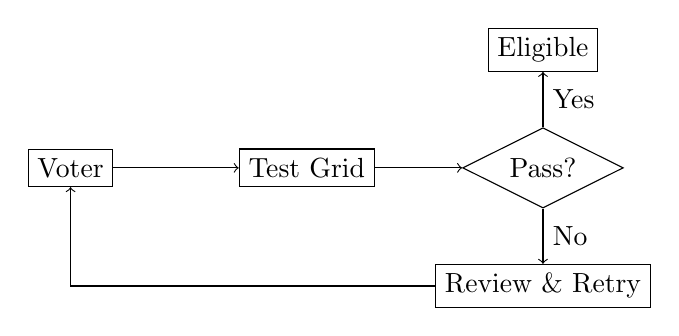
\begin{tikzpicture}[node distance=2cm]
    \node[draw, rectangle] (voter) {Voter};
    \node[draw, rectangle, right of=voter, node distance=3cm] (grid) {Test Grid};
    \node[draw, diamond, right of=grid, node distance=3cm, aspect=2] (pass) {Pass?};
    \node[draw, rectangle, above of=pass, node distance=1.5cm] (eligible) {Eligible};
    \node[draw, rectangle, below of=pass, node distance=1.5cm] (retry) {Review \& Retry};

    \draw[->] (voter) -- (grid);
    \draw[->] (grid) -- (pass);
    \draw[->] (pass) -- node[right] {Yes} (eligible);
    \draw[->] (pass) -- node[right] {No} (retry);
    \draw[->] (retry) -| (voter);
\end{tikzpicture}
\end{center}

The engagement verification does not measure intelligence, political alignment, or
agreement with artifact conclusions. It verifies that the voter has \textit{encountered}
the admissible artifacts relevant to this proposal.

\textbf{Critical clarification}: A voter who has engaged with the evidence and
\textit{disagrees} with its conclusions still passes the gate. The system verifies
engagement, not agreement.

Passing the verification:
\begin{itemize}
    \item Updates the voter's credential NFT (engagements verified counter)
    \item Grants eligibility to vote on this specific proposal
    \item Contributes to the voter's reputation score
\end{itemize}

\textbf{Coherence dimension}: Procedural coherence---voters demonstrate engagement
with relevant artifacts before influencing outcomes.

\subsection{Stage 5: Votes Cast}

Eligible voters cast weighted votes:

\begin{lstlisting}[language=Rust]
// Weight calculation from lib.rs
let base_weight = participant.reputation;
let entropy_factor = (entropy[0] as u64 % 21) as i64 - 10;
let quantum_adjustment = (base_weight as i64 * entropy_factor) / 100;
let final_weight = (base_weight as i64 + quantum_adjustment).max(1);
\end{lstlisting}

Vote weight is a function of:
\begin{enumerate}
    \item \textbf{Reputation}: Accumulated from contributions, engagements verified, prior votes
    \item \textbf{Quadratic cost}: Multiple votes on same proposal cost $n^2$
    \item \textbf{Quantum entropy}: $\pm 10\%$ randomization prevents prediction
\end{enumerate}

Each vote consumes quantum entropy and records a quantum signature.

\textbf{Coherence dimensions}:
\begin{itemize}
    \item Influence coherence (quadratic bounds)
    \item Process coherence (entropy randomization)
\end{itemize}

\subsection{Stage 6: Result}

After the voting period, finalization computes the result:

\begin{lstlisting}[language=Rust]
// The dual condition from lib.rs
let approved = approve_weight > reject_weight
    && quantum_confidence > 50;
\end{lstlisting}

Two conditions must \textbf{both} be satisfied:

\begin{enumerate}
    \item \textbf{Democratic condition}: $w_{\text{approve}} > w_{\text{reject}}$
    \item \textbf{Coherence condition}: $\gamma > 50$
\end{enumerate}

The coherence score $\gamma$ measures entropy variance across votes:
\begin{equation}
    \gamma = \min\left(\frac{\sigma^2_\eta}{255}, 1\right) \times 100
\end{equation}

Low variance indicates correlated votes (Sybil attack, coordination).
High variance indicates independent voting (legitimate process).

\textbf{Critical clarification}: The coherence score measures \textit{process quality},
not outcome correctness. A proposal can pass with high coherence and still be ``wrong''
by external standards. The score measures whether the \textit{process} exhibited
properties consistent with legitimate deliberation, independent of proposal content.

\textbf{Coherence dimension}: Process coherence---the voting process itself
must exhibit properties of statistical independence and adequate entropy.

\subsection{The Integration Point}

The pipeline stages are not independent. Each feeds the next:

\begin{equation}
\text{Credential} \xrightarrow{\text{enables}} \text{Engagement} \xrightarrow{\text{unlocks}} \text{Vote} \xrightarrow{\text{weighted by}} \text{Reputation} \xrightarrow{\text{checked by}} \text{Coherence}
\end{equation}

Specifically:

\begin{itemize}
    \item \textbf{Engagement pass $\rightarrow$ Reputation}: Each verified engagement increments reputation
    \item \textbf{Reputation $\rightarrow$ Vote weight}: Higher reputation = higher base weight
    \item \textbf{Vote weight $\rightarrow$ Coherence}: Weight distribution affects $\gamma$
    \item \textbf{Coherence $\rightarrow$ Credential}: Failed coherence doesn't update credentials
\end{itemize}

This creates a \textit{feedback loop}: good-faith participation builds reputation,
which increases influence, which is checked by coherence, which rewards
legitimate behavior.

\subsection{Why Both Admissibility and Process Coherence}

One might ask: if voters demonstrate artifact engagement, why also check coherence?

The answer: \textbf{they protect against different attacks}.

\begin{center}
\begin{tabular}{lcc}
\toprule
\textbf{Attack} & \textbf{Blocked by Engagement} & \textbf{Blocked by $\gamma$} \\
\midrule
Unengaged voting & \checkmark & --- \\
Sybil (fake identities) & Partial & \checkmark \\
Coordinated manipulation & --- & \checkmark \\
Bribery & --- & \checkmark \\
Credential theft & --- & \checkmark \\
Bot voting & \checkmark & \checkmark \\
\bottomrule
\end{tabular}
\end{center}

\begin{itemize}
    \item \textbf{Admissibility gate} (engagement verification): Ensures voters have \textit{encountered} the relevant artifacts
    \item \textbf{Coherence gate} ($\gamma$): Ensures votes are \textit{statistically independent}
\end{itemize}

A voter who demonstrates engagement but coordinates with others will trigger low $\gamma$.
A voter who votes independently but hasn't engaged with artifacts fails the admissibility gate.
Both gates must pass for legitimate outcomes.

\subsection{The Complete Coherence Invariant}

Combining all dimensions, the system maintains a multi-dimensional coherence invariant:

\begin{definition}[Democratic Coherence]
A proposal outcome is \textbf{democratically coherent} if and only if:
\begin{enumerate}
    \item All voters held valid credentials (credential coherence)
    \item All voters demonstrated artifact engagement (procedural coherence)
    \item Vote weights were bounded by quadratic costs (influence coherence)
    \item Deliberation met minimum duration (temporal coherence)
    \item Entropy distribution showed high variance (process coherence)
    \item Majority of weighted votes approved (democratic condition)
\end{enumerate}
\end{definition}

The system rejects outcomes that satisfy some but not all conditions.
This is the ``coherence preservation'' of the central thesis:

\begin{quote}
\textbf{Democratic legitimacy is a measurable property of process quality,
independent of specific outcomes.}
\end{quote}

Majority rule is necessary but not sufficient. The coherence invariant
must also hold. The system constrains \textit{how} decisions are made,
not \textit{what} decisions must conclude.

\subsection{Pipeline Failure Modes}

Each stage can fail, with different recovery paths:

\begin{center}
\begin{tabular}{lll}
\toprule
\textbf{Stage Failure} & \textbf{Symptom} & \textbf{Recovery} \\
\midrule
1. Invalid submitter & Rejected immediately & Get credential \\
2. Review rejection & Question held & Revise and resubmit \\
3. Grid challenge & Grid invalidated & New curators assigned \\
4. Engagement failure & Voter ineligible & Engage with artifacts, retry \\
5. Vote rejection & Vote not counted & Resubmit with valid sig \\
6. $\gamma \leq 50$ & No state change & Investigate, revote \\
\bottomrule
\end{tabular}
\end{center}

Critically: \textbf{no failure corrupts state}. The system remains at $s_t$
until a coherent transition to $s_{t+1}$ is achieved.

\textbf{Important}: Coherence failure ($\gamma \leq 50$) does not indicate that
the proposal is wrong or harmful. It indicates only that the \textit{process}
exhibited statistical anomalies (coordination, manipulation, or entropy exhaustion).

\subsection{Summary: One Pipeline, Six Coherence Checks}

The augmented democracy system is a single pipeline:

\begin{center}
\fbox{Question $\rightarrow$ Approval $\rightarrow$ Grid $\rightarrow$ Engagement $\rightarrow$ Vote $\rightarrow$ Result}
\end{center}

Each transition is gated by a coherence check:

\begin{center}
\fbox{Credential $\rightarrow$ Temporal $\rightarrow$ Procedural $\rightarrow$ Procedural $\rightarrow$ Influence+Process $\rightarrow$ Process}
\end{center}

The ``underlying current'' is coherence preservation at every stage.
The system is not a voting mechanism with add-ons---it is a coherence-preserving
pipeline that happens to include voting as one stage.

This is the engineering realization of the central thesis: legitimacy
emerges from process invariants, not outcome ratification.

\textbf{The governance system constrains how decisions are made, not what decisions
must conclude.}


%------------------------------------------------------------------------------
\section{Coherence Constraints in Democratic Systems}
\label{sec:coherence-constraints}
%------------------------------------------------------------------------------

\subsection{Coherence Functionals for Proposals}

Let $\mathcal{P}$ be the space of proposals and $\mathcal{C}: \mathcal{P} \rightarrow [0,1]$
a coherence functional. A proposal $p$ is \textit{on-manifold} if $\mathcal{C}(p) > \tau$
for threshold $\tau$.

In the implementation, $\mathcal{C}$ is realized through quantum confidence scoring:
\begin{equation}
    \mathcal{C}(p) = \frac{\gamma_p}{100}
\end{equation}
where $\gamma_p$ is computed from entropy variance across votes on $p$.

\textbf{Important}: $\gamma$ measures process quality, not outcome correctness.
High $\gamma$ indicates statistically independent participation with adequate
entropy. Low $\gamma$ indicates coordination, manipulation, or resource exhaustion.

\subsection{Bounded Influence}

No single participant can dominate outcomes. The weight function satisfies:
\begin{equation}
    w_i \in [w_{\min}, w_{\max}] \quad \forall i
\end{equation}
with $w_{\min} = 1$ (floor) and $w_{\max} = r_i \cdot 1.1$ (reputation cap with 10\% entropy bonus).

\subsection{Rollback and Retry Semantics}

Failed coherence checks do not corrupt state. The system remains at $s_t$ when:
\begin{itemize}
    \item $w_{\text{approve}} \leq w_{\text{reject}}$ (democratic failure)
    \item $\gamma \leq 50$ (coherence failure)
    \item Entropy pool exhausted (resource failure)
\end{itemize}

Submitters may revise and resubmit. The state machine supports retry without penalty.

\subsection{Limited Adversarial Feedback}

The system limits adversarial feedback by restricting rejection signals to typed
errors and coarse-grained status transitions.
While no distributed system can eliminate all side-channel information, this
design prevents gradient-style probing of coherence thresholds and minimizes
adaptive manipulation.

Malicious proposals trigger explicit rejection with typed errors. The error taxonomy
(Section~\ref{sec:governance-control}) ensures that:
\begin{enumerate}
    \item Attackers receive no fine-grained information about \textit{why} rejection occurred
    \item Legitimate users receive actionable feedback via different channels
    \item All rejections are logged for audit
\end{enumerate}

%------------------------------------------------------------------------------
\section{Quantum-Safe and Post-Quantum Alignment}
\label{sec:quantum}
%------------------------------------------------------------------------------

This is not a cryptography paper. However, the governance system inherits quantum resistance
from its substrate:

\subsection{Why Classical Assumptions Fail}

\begin{itemize}
    \item RSA/ECDSA signatures are broken by Shor's algorithm
    \item Hash-based commitments remain secure (Grover provides only quadratic speedup)
    \item Retroactive compromise: adversaries may record today's traffic for future decryption
\end{itemize}

\subsection{Post-Quantum Protections}

The Quantum Harmony implementation uses:
\begin{itemize}
    \item \textbf{SPHINCS+-256s}: Stateless hash-based signatures (NIST PQC standard)
    \item \textbf{Blake2-256}: Quantum-resistant hashing
    \item \textbf{QKD entropy}: True quantum randomness from KIRQ network
\end{itemize}

\subsection{Proof-of-Coherence vs.\ Proof-of-Work/Stake}

\begin{center}
\begin{tabular}{lccc}
\toprule
\textbf{Property} & \textbf{PoW} & \textbf{PoS} & \textbf{PoC} \\
\midrule
Energy cost & High & Low & Low \\
Plutocracy risk & Medium & High & Low \\
Quantum resistance & None & None & Full \\
Sybil resistance & Hash rate & Stake & Coherence \\
Manipulation detection & None & None & Built-in \\
\bottomrule
\end{tabular}
\end{center}

Proof-of-Coherence detects manipulation \textit{before} state transition, whereas PoW/PoS
detect only after finalization (if at all).

%------------------------------------------------------------------------------
\section{Historical Implementation: From Concept to Quantum Infrastructure}
\label{sec:history}
%------------------------------------------------------------------------------

The augmented democracy framework has evolved through eight years of development,
from theoretical conception to production deployment.

\subsection{Conceptual Foundation (2017)}

The original framework was published in August 2017 as ``A Machine-Based Societal
Model for Curbing Citizen Cynicism''~\cite{cormier2017augmented}. Key concepts
established:

\begin{itemize}
    \item \textbf{Test grids}: Voters must demonstrate engagement with relevant evidence
    \item \textbf{Mechanical humans}: Low-barrier contribution tasks for universal participation
    \item \textbf{Operating system metaphor}: Governance as a self-regulating system
    \item \textbf{Blockchain validation}: Immutable record of all decisions
    \item \textbf{Official as safeguard}: Human oversight of machine recommendations
\end{itemize}

The 2017 paper explicitly framed democracy as ``critical infrastructure'' requiring
engineering discipline---a perspective that remains central to the current implementation.

\subsection{EOS Prototype and Oracle Integration (2020--2021)}

The first production implementation deployed as an EOS smart contract:

\begin{itemize}
    \item \textbf{augdemocracy.cpp}: Core smart contract with registration and voting
    \item \textbf{Token Curated Test Grids}: KILT-inspired gatherer/curator structure~\cite{kilt2020}
    \item \textbf{Oracle integration}: Decentralized artifact sourcing via oracle networks
    \item \textbf{Dynamic NFTs}: Early credential management prototypes
    \item \textbf{Quadratic voting}: Whale resistance mechanisms
\end{itemize}

The EOS implementation validated the admissibility gate concept in production,
demonstrating that artifact-engagement verification was technically feasible and user-acceptable.
Concurrent research into Polkadot ecosystem oracle solutions (including Kylin Network,
a Polkadot parachain for cross-chain data feeds) informed the design of the
decentralized artifact-sourcing layer.

\subsection{Substrate Migration (2022--2023)}

Migration to the Substrate framework enabled:

\begin{itemize}
    \item \textbf{Pallet architecture}: Modular, upgradeable governance components
    \item \textbf{Cross-chain compatibility}: Polkadot ecosystem integration
    \item \textbf{Runtime upgrades}: Governance system self-modification
    \item \textbf{Improved NFT standards}: FRAME-native credential tokens
\end{itemize}

The Substrate pallet (\texttt{pallet-quantum-democracy}) preserved all EOS-era
features while adding formal verification capabilities.

\subsection{Quantum Harmony Integration (2024--2025)}

Current production deployment on Quantum Harmony blockchain:

\begin{itemize}
    \item \textbf{Quantum entropy pool}: True randomness from KIRQ network
    \item \textbf{Coherence-based consensus}: Replaces stake-based finality
    \item \textbf{Post-quantum signatures}: SPHINCS+-256s for credential integrity
    \item \textbf{QKD-protected channels}: Quantum key distribution for artifact delivery
    \item \textbf{Toshiba/Crypto4A integration}: Hardware security module support
\end{itemize}

\subsection{Continuity of Core Principles}

Across all implementations, core principles remain constant:

\begin{center}
\begin{tabular}{lcccc}
\toprule
\textbf{Principle} & \textbf{2017} & \textbf{EOS} & \textbf{Substrate} & \textbf{QH} \\
\midrule
Artifact-gated voting & Concept & Implemented & Enhanced & Production \\
Dynamic credentials & Concept & Prototype & NFT-based & Life-sustaining \\
Quadratic bounds & Concept & Implemented & Integrated & + Entropy \\
Coherence threshold & Implicit & Partial & Formal & Quantum \\
Official safeguard & Central & Preserved & Root-only & Emergency \\
\bottomrule
\end{tabular}
\end{center}

This evolution demonstrates that augmented democracy is not speculative---it is
iteratively refined infrastructure with continuous production deployment since 2020.

%------------------------------------------------------------------------------
\section{Failure Modes and Emergency Governance}
\label{sec:failure}
%------------------------------------------------------------------------------

\subsection{When Coherence Fails}

Coherence failure ($\gamma \leq 50$) indicates:
\begin{enumerate}
    \item \textbf{Coordinated attack}: Sybil voters with correlated entropy
    \item \textbf{Entropy exhaustion}: Insufficient quantum randomness
    \item \textbf{System compromise}: Entropy source manipulation
\end{enumerate}

Coherence failure does \textit{not} indicate that the proposal is wrong, harmful,
or should be rejected on substantive grounds. It indicates only that the
\textit{process} exhibited statistical anomalies.

\subsection{Emergency Committee Override}

For critical failures, the system supports:
\begin{lstlisting}[language=Rust]
ensure_root(origin)?;  // Root-only operations
\end{lstlisting}

This is the ``break glass'' mechanism. Root authority can:
\begin{itemize}
    \item Replenish entropy pool
    \item Pause voting
    \item Trigger manual review
\end{itemize}

Root cannot:
\begin{itemize}
    \item Directly approve/reject proposals
    \item Modify vote records
    \item Alter coherence thresholds retroactively
\end{itemize}

\subsection{Human-in-the-Loop Escalation}

When automated coherence checks fail repeatedly, the system escalates to human review:
\begin{enumerate}
    \item Proposal flagged for manual assessment
    \item Validator committee convenes (off-chain)
    \item Committee issues signed recommendation
    \item Recommendation enters normal voting pipeline
\end{enumerate}

This preserves the coherence constraint while acknowledging that some edge cases
require human judgment.

\subsection{Response Windows}

\begin{center}
\begin{tabular}{lcc}
\toprule
\textbf{Event} & \textbf{Detection} & \textbf{Response} \\
\midrule
Low entropy & Immediate & Auto-pause voting \\
Coherence failure & At finalization & Proposal held \\
Repeated failures & 3 consecutive & Escalate to committee \\
System compromise & Manual detection & Emergency halt \\
\bottomrule
\end{tabular}
\end{center}

%------------------------------------------------------------------------------
% User Experience and Agent Delegation
%------------------------------------------------------------------------------
\section{User Experience: Hiding the Machinery}
\label{sec:ux}

The preceding sections describe protocol mechanics. This section addresses the
critical question: \textit{how does a citizen actually use this?}

The coherence pipeline has six stages and multiple credential types. Exposing this
complexity to end users would guarantee adoption failure. The system must feel
like ``just voting'' while the coherence machinery runs invisibly beneath.

\subsection{The TCP/IP Principle}

Users do not understand TCP/IP, TLS handshakes, or DNS resolution. They ``browse
the web.'' The complexity exists but is entirely hidden by the browser interface.

Augmented democracy requires the same architectural separation:

\begin{center}
\begin{tabular}{ll}
\toprule
\textbf{Layer} & \textbf{What User Sees} \\
\midrule
Protocol & (invisible) \\
Application & Simple voting interface \\
Experience & ``I voted on the transit proposal'' \\
\bottomrule
\end{tabular}
\end{center}

The test grids, NFT credentials, quadratic costs, and coherence thresholds operate
at the protocol layer. The user interacts with the application layer.

\subsection{The Streamlined Experience}

For a typical citizen voting on a local issue:

\begin{enumerate}
    \item \textbf{Open app, see proposals}: ``New transit line proposal''
    \item \textbf{Tap to learn more}: 2-minute summary video + key information
    \item \textbf{Quick quiz appears}: 3 questions, multiple choice
    \item \textbf{Pass quiz}: ``You're ready to vote!''
    \item \textbf{Vote}: Approve / Reject / Abstain
    \item \textbf{Done}: ``Your vote is recorded''
\end{enumerate}

Total time: \textbf{4 minutes}.

What happened invisibly:
\begin{itemize}
    \item App checked credential NFT validity
    \item Quiz was the engagement verification grid (presented as ``quick quiz'')
    \item Pass threshold was applied
    \item Vote was signed with quantum signature
    \item Quadratic cost was calculated (first vote = 1 token, shown as ``free'')
    \item Vote entered coherence pool
\end{itemize}

The user experienced: ``watched video, answered quiz, voted.''

\subsection{Progressive Disclosure}

Different users need different depth:

\begin{center}
\begin{tabular}{lll}
\toprule
\textbf{User Type} & \textbf{Sees} & \textbf{Hidden} \\
\midrule
Casual voter & Quiz + vote button & Everything else \\
Engaged citizen & Reputation score, vote history & NFT mechanics \\
Power user & Credential details, weight calc & Protocol internals \\
Curator & Grid builder interface & Consensus mechanics \\
Developer & Full protocol access & Nothing \\
\bottomrule
\end{tabular}
\end{center}

The interface progressively reveals complexity only when users seek it.

\subsection{The Quiz Is the Engagement Verification}

The ``test grid'' sounds bureaucratic. The experience is:

\begin{quote}
``Before you vote, let's make sure you've seen the key information.
Here are 3 quick questions.''
\end{quote}

The questions verify engagement with the evidence:
\begin{itemize}
    \item ``The proposed transit line would cost approximately: (a) \$2B (b) \$5B (c) \$10B''
    \item ``The project timeline is: (a) 2 years (b) 5 years (c) 10 years''
    \item ``The main opposition concern is: (a) cost (b) displacement (c) noise''
\end{itemize}

\textbf{Critical clarification}: This is not an IQ test or agreement test.
It verifies the voter has \textit{encountered} the relevant information.
A voter who has engaged with the evidence and \textit{disagrees} with it
still passes. The system verifies engagement, not agreement.

Failing means: ``Review the summary and try again'' --- not punishment, just
a nudge to engage with the material.

\subsection{Credential Management Is Invisible}

Users never see ``NFT credential'' language. They see:

\begin{itemize}
    \item \textbf{Account creation}: ``Sign up with email'' (NFT minted in background)
    \item \textbf{Reputation}: ``Your civic score: 127'' (reputation field)
    \item \textbf{Eligibility}: ``You can vote on 12 active proposals'' (credential check)
    \item \textbf{Decay warning}: ``Vote this month to keep your streak!'' (vitality)
\end{itemize}

The gamification layer (scores, streaks, badges) maps directly to protocol
primitives (reputation, vitality, domain credentials) without exposing the
underlying mechanics.

\subsection{Quadratic Costs as ``Voting Power''}

Quadratic voting sounds academic. The UX:

\begin{quote}
``You have 100 voting power this month.''\\
``Spending 1 power = 1 vote.''\\
``Spending 4 power = 2 votes (for issues you care deeply about).''\\
``Spending 9 power = 3 votes.''
\end{quote}

Users understand ``spend more to vote stronger on things you care about.''
The quadratic cost is implicit in the power/vote ratio.

Most users spend 1 power per proposal and never think about the math.

\subsection{The Curator Path}

For users who want deeper engagement, the curator path opens:

\begin{enumerate}
    \item \textbf{Contribute sources}: ``Add a source document to this proposal''
    \item \textbf{Build quizzes}: ``Write a question for this proposal''
    \item \textbf{Earn tokens}: ``You earned 5 tokens for your contribution''
    \item \textbf{Gain reputation}: ``Your civic score increased to 142''
\end{enumerate}

Curators experience the system as a contribution platform with rewards.
The staking, slashing, and credential mechanics are protocol-level concerns.

\subsection{Failure States as Friendly Nudges}

Protocol failures translate to friendly UX:

\begin{center}
\begin{tabular}{ll}
\toprule
\textbf{Protocol State} & \textbf{User Message} \\
\midrule
Engagement not verified & ``Review the summary and try the quiz again'' \\
Credential expired & ``Welcome back! Quick verification needed'' \\
Insufficient power & ``You've used your voting power this month'' \\
Coherence failure & ``This vote is under review---we'll notify you'' \\
\bottomrule
\end{tabular}
\end{center}

No user ever sees ``InsufficientQuantumEntropy'' or ``CoherenceThresholdNotMet.''

\subsection{The 2017 Vision: Comfortable Contribution}

The original 2017 paper emphasized that contribution must be ``comfortable'':

\begin{quote}
``An individual must be granted the freedom to choose their level of involvement,
the type of involvement they want to partake in, and the level of privacy they
want for a particular transaction.''
\end{quote}

This translates to:
\begin{itemize}
    \item \textbf{Level of involvement}: Casual voter vs. curator vs. developer
    \item \textbf{Type of involvement}: Vote, contribute sources, build quizzes, write code
    \item \textbf{Privacy level}: Public reputation vs. anonymous mode
\end{itemize}

The system accommodates all engagement levels without forcing complexity on
those who don't want it.

\subsection{Mobile-First, 4-Minute Sessions}

The target interaction:

\begin{itemize}
    \item \textbf{Platform}: Mobile app (iOS/Android)
    \item \textbf{Session length}: 2--5 minutes
    \item \textbf{Notification}: ``3 proposals need your vote this week''
    \item \textbf{Interaction}: Watch summary $\rightarrow$ quiz $\rightarrow$ vote
    \item \textbf{Reward}: ``+5 civic score, streak maintained''
\end{itemize}

This is the friction target: \textbf{less friction than checking social media}.

\subsection{Incentive Alignment}

Why would anyone participate?

\begin{center}
\begin{tabular}{ll}
\toprule
\textbf{Incentive} & \textbf{Mechanism} \\
\midrule
Civic score & Social status, visible to others \\
Streaks & Gamification, loss aversion \\
Token rewards & Direct compensation for curation \\
Influence & Higher reputation = more vote weight \\
Tax benefits & Civic contribution deductions (policy) \\
\bottomrule
\end{tabular}
\end{center}

The 2017 paper proposed that civic contribution could offset taxes and
unlock social benefits. The exact incentive structure is policy, not protocol---
but the protocol supports any incentive model.

\subsection{Summary: The Experience Stack}

\begin{center}
\begin{tabular}{ll}
\toprule
\textbf{Layer} & \textbf{Contents} \\
\midrule
\textbf{Experience} & ``I voted on transit'' \\
\textbf{Interface} & Quiz, vote button, score display \\
\textbf{Application} & Credential check, weight calc, submission \\
\textbf{Protocol} & NFTs, entropy, signatures, coherence \\
\textbf{Consensus} & Quantum Harmony blockchain \\
\bottomrule
\end{tabular}
\end{center}

The protocol is complex. The experience is simple.

This is the same pattern as the modern web: users don't understand HTTPS,
but they trust the lock icon. Users won't understand coherence thresholds,
but they'll trust ``Your vote is verified.''

The machinery serves the experience. Not the reverse.

\subsection{Agent-Mediated Participation}

The preceding subsections assume human users navigating a simplified interface.
A more radical approach: \textbf{delegate to AI agents}.

Humans don't navigate TCP/IP because \textit{browsers} do it for them. Similarly,
humans may not navigate the coherence pipeline because \textit{agents} do it
for them.

\subsubsection{What Agents Can Do}

An AI agent operating on behalf of a citizen can:

\begin{itemize}
    \item \textbf{Monitor proposals}: ``3 new proposals match your interests''
    \item \textbf{Summarize content}: Digest 50-page proposals into 2-minute briefings
    \item \textbf{Complete engagement verifications}: Parse test grids and demonstrate artifact engagement
    \item \textbf{Maintain credentials}: Ensure NFT vitality, renew before decay
    \item \textbf{Calculate spending}: Optimize quadratic voting across proposals
    \item \textbf{Vote within bounds}: Execute votes per user-defined preferences
    \item \textbf{Track coherence}: Alert user if coherence scores are anomalous
\end{itemize}

The human experience becomes:

\begin{enumerate}
    \item \textbf{Set preferences}: ``I care about transit, housing, environment''
    \item \textbf{Review agent recommendations}: ``Your agent suggests: Approve transit, Reject rezoning''
    \item \textbf{Confirm or override}: Tap to accept, or dive deeper
    \item \textbf{Done}: Agent handles everything else
\end{enumerate}

Total human time: \textbf{30 seconds per week}.

\subsubsection{Delegation Bounds}

Agents operate within \textit{delegation bounds} set by the user:

\begin{lstlisting}[language=Rust]
pub struct DelegationBounds {
    // What the agent CAN do autonomously
    pub can_complete_engagements: bool,
    pub can_vote_low_stakes: bool,  // < threshold
    pub can_manage_credentials: bool,

    // What requires human confirmation
    pub vote_threshold: Balance,    // Above this, ask human
    pub domains_excluded: Vec<Domain>, // Never vote on these
    pub require_confirmation: bool, // Always ask before voting

    // Limits
    pub max_daily_votes: u32,
    pub max_weekly_spend: Balance,
}
\end{lstlisting}

A conservative user might set: ``Agent can complete engagement verifications, but always ask me before voting.''

A trusting user might set: ``Agent can vote on anything under 10 tokens; ask me for high-stakes only.''

\subsubsection{Agent Accountability}

Critical question: \textit{who is accountable for agent actions?}

The answer: \textbf{the human principal}.

\begin{itemize}
    \item Agent actions are signed with the human's credential
    \item Vote history shows ``voted via agent'' flag
    \item Reputation changes accrue to the human
    \item The human remains accountable for agent behavior
\end{itemize}

The agent is a tool, not a participant. The human delegates but remains accountable.

\subsubsection{Agent Coherence (ERLHS Connection)}

If agents vote, the agents themselves need coherence constraints.

This connects directly to ERLHS~\cite{cormier2025erlhs}: the Hamiltonian framework
for coherence-preserving machine intelligence. An agent operating in the
augmented democracy system should:

\begin{itemize}
    \item Maintain internal state coherence (ERLHS constraint)
    \item Respect delegation bounds (policy constraint)
    \item Produce auditable reasoning (transparency constraint)
    \item Avoid manipulation of other agents (adversarial constraint)
\end{itemize}

The coherence requirements apply at two levels:
\begin{enumerate}
    \item \textbf{Democratic coherence}: The voting system (this paper)
    \item \textbf{Agent coherence}: The AI operating within it (ERLHS)
\end{enumerate}

\subsubsection{Mass Agent Attacks}

New threat model: adversary deploys many agents to vote in coordinated patterns.

Defenses:
\begin{itemize}
    \item \textbf{Coherence detection}: Coordinated agents produce low entropy variance ($\gamma$)
    \item \textbf{Agent diversity requirements}: Agents must demonstrate behavioral variance
    \item \textbf{Human-in-loop checkpoints}: High-stakes votes require human confirmation
    \item \textbf{Agent registration}: Agents themselves may need credentials
\end{itemize}

The quantum confidence score $\gamma$ was designed to detect Sybil attacks.
It also detects coordinated agent behavior---agents voting in lockstep
produce low variance, triggering coherence failure.

\subsubsection{The Agent-Native Interface}

For agent-mediated participation, the ``interface'' is an API:

\begin{lstlisting}[language=Rust]
trait AgentInterface {
    fn get_proposals(&self, filters: ProposalFilters)
        -> Vec<ProposalSummary>;
    fn get_engagement_grid(&self, proposal_id: u32)
        -> EngagementGrid;
    fn submit_engagement_answers(&self, proposal_id: u32, answers: Vec<Answer>)
        -> EngagementResult;
    fn cast_vote(&self, proposal_id: u32, vote: VoteType, weight: u64)
        -> VoteReceipt;
    fn get_coherence_status(&self, proposal_id: u32)
        -> CoherenceStatus;
}
\end{lstlisting}

Human-facing apps and agent systems use the same underlying protocol.
The difference is who drives the interaction.

\subsubsection{The Future: Humans Set Values, Agents Execute}

The end state:

\begin{center}
\begin{tabular}{ll}
\toprule
\textbf{Human Role} & \textbf{Agent Role} \\
\midrule
Set values and priorities & Monitor proposal stream \\
Review agent recommendations & Summarize and analyze \\
Confirm high-stakes votes & Execute routine votes \\
Override when needed & Maintain credentials \\
Remain accountable & Optimize participation \\
\bottomrule
\end{tabular}
\end{center}

This is not ``AI voting instead of humans.'' It is ``AI handling friction
so humans can focus on values.''

The human remains the principal. The agent is the instrument.
The coherence constraints apply to both.

\textbf{The governance system constrains how decisions are made, not what decisions
must conclude.}


%------------------------------------------------------------------------------
\section{Conclusion: Democracy as Infrastructure}
\label{sec:conclusion}
%------------------------------------------------------------------------------

Democracy is no longer a philosophical abstraction. It is \textbf{critical infrastructure}.

The systems we use to make collective decisions are under adversarial load from state actors,
AI-generated influence, and the fundamental speed/quality tradeoff of digital communication.
Traditional democratic theory offers no defense against these threats because it treats
legitimacy as a property of outcomes rather than processes.

This paper has presented an alternative: \textit{coherence-constrained democratic systems}
with \textit{procedural infrastructure}, where:
\begin{enumerate}
    \item Proposals are state transitions in a formal control system
    \item Participants hold dynamic credentials that evolve with contribution
    \item Voters must demonstrate engagement with admissible artifacts (procedural gate)
    \item Quadratic voting costs bound plutocratic influence
    \item Deliberation is a filtering operation with minimum dwell time
    \item Approval requires both majority support \textit{and} coherence threshold
    \item All transitions produce cryptographic proofs
    \item Credentials decay without ongoing participation (life-sustaining NFTs)
\end{enumerate}

The central thesis is that \textbf{democratic legitimacy is a measurable property of
process quality, independent of specific outcomes}.

This is not ideology. It is engineering.

\textbf{The governance system constrains how decisions are made, not what decisions
must conclude.}

The framework has evolved through eight years of development---from the 2017 conceptual
paper through EOS smart contract prototypes to the current Quantum Harmony implementation.
Each iteration validated core principles while adding cryptographic hardening. Combined
with prior work on ERLHS (coherence in AI), Karmonic Mesh (geometric substrate), and
Proof of Coherence (distributed validation), this framework provides a complete architecture
for augmented democracy as 21st-century infrastructure.

The procedural stack---token-curated test grids, dynamic credential NFTs, quadratic voting,
coherence thresholds, and accountability mechanisms---transforms voting from opinion
aggregation into \textit{structured preference revelation}. This is the augmentation that
gives augmented democracy its name: not technological enhancement of voting mechanics,
but procedural elevation of participation quality.

The friction inherent in this architecture is addressed through agent-mediated
participation: AI agents that navigate the coherence pipeline on behalf of human
principals. Humans set values and priorities; agents handle the mechanics. This
creates a new division of labor---humans as value-setters, agents as executors---
with coherence constraints applying at both levels. The ERLHS framework ensures
agent coherence; the democratic framework ensures process coherence. Together,
they enable participation at scale without sacrificing procedural quality.

The ultimate vision: a system where legitimate collective decisions emerge from
coherence-preserving processes, mediated by trustworthy agents, grounded in
verifiable artifacts, and accountable to human values. This is democracy as infrastructure---
engineered, deployable, and resistant to adversarial conditions.

%------------------------------------------------------------------------------
% References
%------------------------------------------------------------------------------
\bibliographystyle{plain}
\begin{thebibliography}{99}

\bibitem{cormier2017augmented}
Cormier, S. (2017).
\textit{A Machine-Based Societal Model for Curbing Citizen Cynicism}.
Unpublished manuscript, August 2017.

\bibitem{cormier2025erlhs}
Cormier, S. (2025).
\textit{ERLHS: A Hamiltonian Framework for Coherence-Preserving Machine Intelligence}.
Zenodo. \url{https://doi.org/10.5281/zenodo.17928909}

\bibitem{cormier2025karmonic}
Cormier, S. (2025).
\textit{Karmonic Mesh: Spectral Consensus on Toroidal Manifolds}.
Zenodo. \url{https://doi.org/10.5281/zenodo.17928991}

\bibitem{cormier2025poc}
Cormier, S. (2025).
\textit{Proof of Coherence: QKD-Based Distributed Consensus}.
Zenodo. \url{https://doi.org/10.5281/zenodo.17929054}

\bibitem{cormier2025toroidal}
Cormier, S. (2025).
\textit{Toroidal Mesh: 10K TPS with SPHINCS+ via Parallel Verification}.
Zenodo. \url{https://doi.org/10.5281/zenodo.17931222}

\bibitem{cormier2025governance}
Cormier, S. (2025).
\textit{Toroidal Governance: Tonnetz Manifold Democratic Infrastructure}.
Zenodo. \url{https://doi.org/10.5281/zenodo.17929091}

\bibitem{buterin2019quadratic}
Buterin, V., Hitzig, Z., \& Weyl, E. G. (2019).
\textit{A Flexible Design for Funding Public Goods}.
Management Science, 65(11), 5171--5187.

\bibitem{kilt2020}
BOTLabs GmbH. (2020).
\textit{KILT Protocol White Paper: Credentials for Web 3.0}.
Berlin, Germany.
\url{https://kilt-protocol.org/files/KILT-White-Paper.pdf}

\end{thebibliography}

\end{document}
